\chapter[Lecture 10]{}\label{lec10}

Full rotation group is the symmetry group of an isolated atom. Orientational degeneracy can be lifted by putting it in a erystalline environment $\to$ BeThe

\section*{Application of Group Theory}

\noindent
{\bf Crystalline solid:}

Lattice is invariant under translation
$$
T=\sum\limits_{i}n_{i}a_{i}\quad a_{i}\to \text{ Primitive translation vectors.}
$$

The other covering operation are rotations, reflections and inversion.

\noindent
{\bf Space group:} Complete set of covering operations - 230 space groups.

\noindent
{\bf Point group:} Covering operations excluding translation.
$$
-32\text{ point groups}
$$

Molecule $\to$ translational symmetry not required. Often 32 point groups are enough to capture symmetry.

\section*{Successive operations}
\begin{itemize}
\item Product of two rotation is a rotation.

\item Product of two reflection about planes $A$ and $B$ is a rotation by $2\phi_{AB}$; $\phi_{AB}$ angle between $A$ and $B$.

\item Product of a rotation and a reflection about $A$ containing the axis of rotation $0$ is a reflection about a plane $B$ intersecting along $0$ with plane $A$ and at an angle half of the angle of rotation.

\item Product of two rotations by $\pi$ about intersecting axis $u$ and $v$ is another rotation about an axis perpendicular to $u$ and $v$; angle of rotation is twice the angle between $u$ and $v$.

\begin{minipage}[c]{5.3cm}
\begin{figure}[H]
\centering
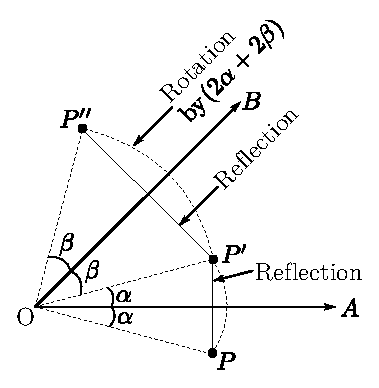
\includegraphics[scale=.8]{images/lecture10/fig2.eps}
\end{figure}
\end{minipage}
\qquad
\begin{minipage}[c]{5.3cm}
\begin{figure}[H]
\centering
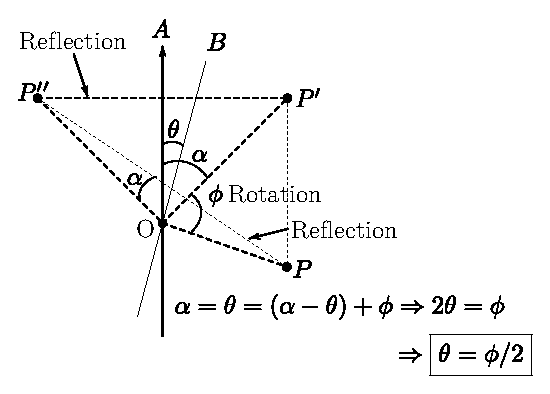
\includegraphics[scale=.8]{images/lecture10/fig3.eps}
\end{figure}
\end{minipage}
\end{itemize}

\section*{Commuting Operations}
\begin{itemize}
\itemsep=0pt
\item[(i)] Two rotation about same axis.

\item[(ii)] Two reflection in perpendicular plane.

\item[(iii)] Two rotation by $\pi$ about perpendicular axes.

\item[(iv)] A rotation and a reflection in a plane perpendicular to rotation axis $\Rightarrow$ improper rotation or rotary reflection.
\end{itemize}
Improper rotation by $\pi$ is $\equiv$ {\bf inversion}.

\section*{Notations}

\noindent
{\bf Schoenflies notation:}
\begin{description}
\itemsep=0pt
\item[$E$] - identity.

\item[$C_{n}$] - rotation through $\dfrac{2\pi}{n}$\quad $n=1,2,3,4,6$.

\item[$\sigma$] - reflection in a plane.

\item[$\sigma_{h}$] $\to$ reflection in the {\bf horizontal} plane; perpendicular to the axis of highest rotation symmetry.

\item[$\sigma_{v}$] $\to$ reflection in vertical plane.

\item[$\sigma_{d}$] $\to$ reflection in a diagonal plane $\to$ the one containing the symmetry axis and bisecting angle between two-fold axes perpendicular to the symmetry axis $-$ a special case of $\sigma_{v}$.

\item[$S_{n}$] $\to$ improper rotation through $\dfrac{2\pi}{n}$.

\item[$i$] $\to$ $=S_{2}=$ inversion.
\end{description}

\noindent
{\bf Two special symmetry operations}
\begin{itemize}
\item[(i)] Screw axes : Translation through a vector not in Bravais lattice (say $t'e_{z}$) followed by a rotation about $Z$-axis defined by translation.

\item[(ii)] Glide planes : Translation through a vector not in Bravais lattice (say $t'e_{z}$) followed by a reflection in a plane containing that vector (say $k-y$ plane)
\end{itemize}

\section*{Inter-relation of symmetry operation}
\begin{description}
\item[1.(a)] Intersection of two reflection planes must be a symmetry axis. If the angle between the planes is $\dfrac{\pi}{n}$, the axis is $n$-fold.

\item[1.(b)] If a reflection plane contains an $n$-fold axis, there must be $(n-1)$ other reflection planes at angles of $\dfrac{\pi}{n}$.

\item[2.(a)] Two $2$-fold axis separated by an angle $\dfrac{\pi}{n}$ require a perpendicular $n$-fold axis.

\item[2.(b)] A two-fold axis and an $n$-fold axis perpendicular to it require $(n-1)$ additional two-fold axis separated by `$\dfrac{\pi}{n}$'.

\item[3.] An even-fold axis, a reflection plane perpendicular to it, and an inversion center are interdependent. Any two of these elements implies presence of the third one.
\end{description}

\section*{Crystallographic Point Group}

\noindent
{\bf Stereographic Projection:} Projection of a point on unit sphere an my-plane which undergoes symmetry operations. $+ \ \to$ above the plane $0 \ \to$ below the plane.

$C_{n} \ \to$ group with single $n$-fold rotation axis. These are cyclic group. e.g., $C_{6},(C_{6})^{2}=C_{3}$, $(C_{6})^{3}=C_{2}$, $(C_{6})^{4}=C^{-1}_{3}$, $(C_{6})^{5}=C^{-1}_{6}$ and $(C_{6})^{6}=E$.

$n=1,2,3,4$ and $6$ are possible.

\begin{proof}
\begin{itemize}
\item[(i)] Assume $R$ is a lattice translation vector after rotation by $\dfrac{2\pi}{n}$ it becomes $R'$.
\begin{figure}[H]
\centering

\includegraphics[scale=.9]{images/lecture10/fig4.eps}
\end{figure}
The difference $|R-R'|$ must be at least $|R|$
\begin{align*}
\therefore\quad 2|R|\sin \dfrac{\pi}{n} &\geq |R|\\
a,\quad \sin \dfrac{\pi}{n} &\geq \dfrac{1}{2}=\sin \dfrac{\pi}{6}\quad \therefore \fbox{$n\leq 6$}
\end{align*}
\begin{figure}[H]
\centering
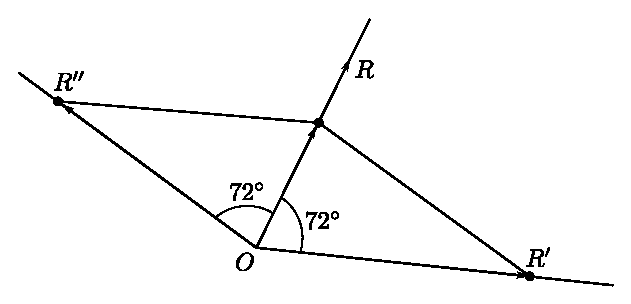
\includegraphics[scale=.9]{images/lecture10/fig5.eps}
\end{figure}

\item[(ii)] Now rotate $R$ by $\dfrac{2\pi}{5}$ in both direction as in figure. We find $|R'+R''|<|R|$ which is not allowed, $\therefore$ \ \fbox{$n\neq 5$}
\end{itemize}

$D_{nd}$: These contain the elements of $D_{n}$ plus $n$ mirror planes containing the $n$-fold axis, which bisect the angles between neighbor twofold axes in $D_{n}$.

It is instructive to verify that the objects shown in Table 2.2 do indeed have the symmetries required by their Schoenflies names.
\end{proof}

\section*{International notation for the noncubic crystallographic point groups}

The international categories are illustrated by grouping the rows in Table 2.2 according to the labels given on the right side. These categories are identical to the Schoenflies categories:

$n$ is the same as $C_{n}$.

$nmm$ is the same as $C_{nv}$. The two $m_{s}$ refer to two distinct types of mirror planes containing the $n$-fold axis. What they are is evident from the illustrating $6mm$, $4mm$, and $2mm$. These demonstrate that a $2j$-fold axis takes a vertical mirror plane into $j$ mirror planes, but in addition, other $j$ mirror planes automatically appear, bisecting the angles between adjacent planes in the first set. However, a $2j+1$-fold axis takes a mirror plane into $2j+1$ equivalent ones, and therefore\footnote{In emphasizing the differences between odd- and even-fold axes, the international system, unlike the Schoenflies, treats the threefold axis as a special case.} $C_{3v}$ is only called $3m$.

$n22$ is the same as $D_{n}$. The discussion is the same as for $nmm$, but now perpendicular twofold axes are involved instead of vertical mirror planes.

$n/m$ is the same as $C_{nh}$, {\em except} that the international system prefers to regard $C_{3h}$ as containing a sixfold rotation-inversion axis, making it $\overline{6}$ (see the next category). Note also that $C_{1h}$ (or called $C_{2i}$) becomes simply $m$, rather than $1/m$.

$S_{n} \ \to$ rotation and reflection in plane perp. to refn. axis.

$\overline{n}$ is a group with an $n$-fold rotation-inversion axis. This category contains $C_{3h}$, disguised as $\overline{6}$. It also contains $S_{4}$, which becomes simple $\overline{4}$. However, $S_{6}$ becomes $\overline{3}$ and $S_{2}$ becomes $\overline{1}$ by virtue of the difference between rotation-reflection and rotation-inversion axes.

$\frac{n}{m}\frac{2}{m}\frac{2}{m}$, abbreviated as $n/mmm$, is just $D_{nh}$, {\em except} that the international system prefers to regard $D_{3h}$ as containing a sixfold rotation-inversion axis, making it $\overline{6}2m$ (see the next category and note the similarity to the ejection of $C_{3h}$ from $n/m$ to $\overline{n}$). Note also that $2/mmm$ is conventionally abbreviated further into $mmm$. The full-blown international title is supposed to remind one that $D_{nh}$ can be viewed as an $n$-fold axis with a perpendicular mirror plane, festooned with two sets of perpendicular twofold axes, each with its own perpendicular mirror planes.

\section*{\em Nomenclature for the cubic crystallographic point groups}

The Schoenflies and international name for the five cubic groups are given in Table 2.1.

$O$ is the cubic (or octahedral, whence the $O$) group, including three fourfold axes $(\langle 100\rangle)$, four threefold axes $(\langle 111\rangle)$, and six twofold axes $(\langle 110 \rangle)$.

$O_{h}$ is the full symmetry group of the cube (or octahedral). It contains the elements of $O$ plus an inversion, including {\em improper} operations.\footnote{Any operation that takes a right-handed object into a left-handed one is called {\em improper} and all others are proper. Operations containing an odd number of inversions or mirrorings are improper.}

$T$ is the group of the regular tetrahedron in Fig.~2.3(b), including four threefold axes $(\langle 111\rangle)$ and three twofold axes $(\langle 100\rangle)$, which connect the midpoints of the opposite edges in the tetrahedron.

$T_{d}$ is the full symmetry group of the regular tetrahedron, including all improper operations. It contains the elements of $T$ plus six mirror planes along $\{110\}$.

$T_{h}$ is what results when an inversion is added to $T$.

The international names for the cubic groups are conveniently distinguished from those of the other crystallographic point groups by containing 3 as a second number, referring to the threefold axis present in all the cubic groups.

\section*{The 230 Space Groups}

The main target of solid state physics is to understand the properties of matter based on the atomic and electronic structures; therefore, the simple structures introduced in Chapter 1 are more suitable for this target. However, most of the materials have much which is not allowed. 

$\therefore \ $ \fbox{$n\neq 5$}
\begin{figure}[H]
\centering
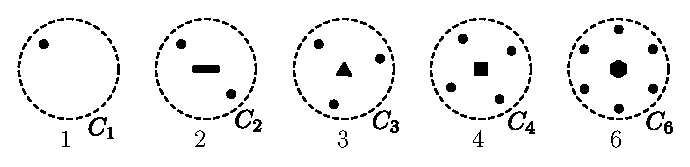
\includegraphics{images/lecture10/fig6.eps}
\end{figure}
\begin{figure}[H]
\centering
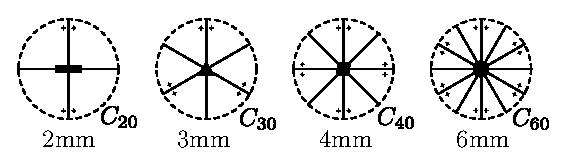
\includegraphics{images/lecture10/fig7.eps}

\bigskip

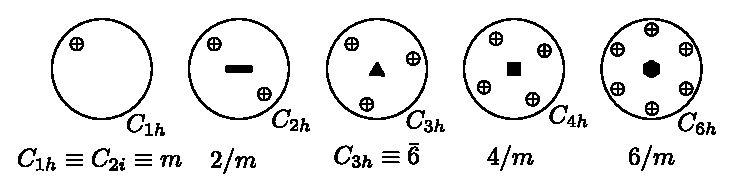
\includegraphics{images/lecture10/fig8.eps}

\bigskip


\includegraphics{images/lecture10/fig9.eps}

\bigskip


\includegraphics{images/lecture10/fig10.eps}

\bigskip

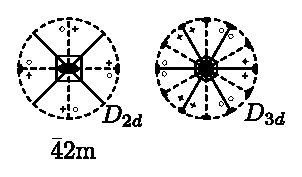
\includegraphics{images/lecture10/fig11.eps}

\bigskip

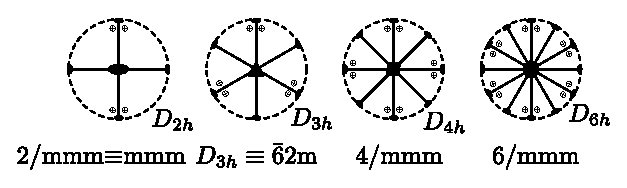
\includegraphics{images/lecture10/fig12.eps}

\caption{Stereographic projections of simple point groups}
\end{figure}



 



